\begin{filecontents}[overwrite]{refs.bib}
@article{safe2025,
  author  = {da Silva Garcia Leite, L. and Zhang, B. and Acar, Z. and Elowitt, J.
             and Augustine, L. J. and Clark, A. E. and Yang, P.},
  title   = {Creation of the Separation Archive for Elements ({SAFE}) Database},
  journal = {Solvent Extraction and Ion Exchange},
  volume  = {43}, number = {7}, pages = {847--852}, year = {2025},
  doi     = {10.1080/07366299.2025.2564381}
}
@article{shannon1976,
  author  = {Shannon, R. D.},
  title   = {Revised Effective Ionic Radii and Systematic Studies of Interatomic
             Distances in Halides and Chalcogenides},
  journal = {Acta Crystallographica Section A},
  volume  = {32}, number = {5}, pages = {751--767}, year = {1976},
  doi     = {10.1107/S0567739476001551}
}
@article{cheisson2019,
  author  = {Cheisson, Thibault and Schelter, Eric J.},
  title   = {Rare earth elements: {M}endeleev's bane, modern marvels},
  journal = {Science},
  volume  = {363}, pages = {489--493}, year = {2019},
  doi     = {10.1126/science.aau7628}
}
@article{bannwarth2019gfn2,
  author  = {Bannwarth, Christoph and Ehlert, Sebastian and Grimme, Stefan},
  title   = {{GFN2-xTB} --- An Accurate and Broadly Parametrized Self-Consistent
             Tight-Binding Quantum Chemical Method with Multipole Electrostatics
             and Density-Dependent Dispersion Contributions},
  journal = {Journal of Chemical Theory and Computation},
  volume  = {15}, number = {3}, pages = {1652--1671}, year = {2019},
  doi     = {10.1021/acs.jctc.8b01176}
}
@misc{gxtb,
  author = {Froitzheim, Thomas and M{\"u}ller, Marcel and Hansen, Andreas and Grimme, Stefan},
  title  = {{g-xTB}: A General-Purpose Extended Tight-Binding Electronic Structure
            Method for the Elements {H} to {Lr} ({Z} = 1--103)},
  howpublished = {ChemRxiv},
  year   = {2025},
  doi    = {10.26434/chemrxiv-2025-bjxvt}
}
@article{lnxtb2026,
  author  = {Zhang, Yang-Yang},
  title   = {New Optimized Parameters of Extended Tight-Binding Method {Ln-xTB}
             ({Ln} = {La}--{Lu}) to Explore Lanthanide Molecular Chemistry},
  journal = {Journal of Computational Chemistry},
  year    = {2026},
  doi     = {10.1002/jcc.70321}
}
@article{architector,
  author  = {Taylor, Michael G. and Burrill, Daniel J. and Janssen, Jan and
             Batista, Enrique R. and Perez, Danny and Yang, Ping},
  title   = {Architector for High-Throughput Cross-Periodic Table {3D}
             Complex Building},
  journal = {Nature Communications},
  volume  = {14}, pages = {2786}, year = {2023},
  doi     = {10.1038/s41467-023-38169-2}
}
@inproceedings{catboost2018,
  author    = {Prokhorenkova, Liudmila and Gusev, Gleb and Vorobev, Aleksandr and
               Dorogush, Anna Veronika and Gulin, Andrey},
  title     = {{CatBoost}: Unbiased Boosting with Categorical Features},
  booktitle = {Advances in Neural Information Processing Systems (NeurIPS)},
  year      = {2018}
}
@inproceedings{schnet2017,
  author    = {Sch{\"u}tt, Kristof T. and Kindermans, Pieter-Jan and
               Sauceda, Huziel E. and Chmiela, Stefan and Tkatchenko, Alexandre
               and M{\"u}ller, Klaus-Robert},
  title     = {{SchNet}: A Continuous-Filter Convolutional Neural Network for
               Modeling Quantum Interactions},
  booktitle = {Advances in Neural Information Processing Systems (NeurIPS)},
  year      = {2017}
}
@article{rogers2010,
  author  = {Rogers, David and Hahn, Mathew},
  title   = {Extended-Connectivity Fingerprints},
  journal = {Journal of Chemical Information and Modeling},
  volume  = {50}, pages = {742--754}, year = {2010},
  doi     = {10.1021/ci100050t}
}
@book{vovk2005,
  author    = {Vovk, Vladimir and Gammerman, Alexander and Shafer, Glenn},
  title     = {Algorithmic Learning in a Random World},
  publisher = {Springer},
  year      = {2005}
}
\end{filecontents}

\documentclass{article}
\usepackage{log_2022}

\usepackage{booktabs}
\usepackage{graphicx}
\usepackage{url}
\usepackage[numbers,compress,sort]{natbib}

\graphicspath{{figures/}}

\makeatletter
\renewcommand{\@noticestring}{%
  Massachusetts Institute of Technology --- Molecular Machine Learning
  Conference 2026.%
}
\makeatother

\newcommand{\logD}{\ensuremath{\log D}}
\newcommand{\logSF}{\ensuremath{\log \mathrm{SF}}}
\newcommand{\adjR}{\ensuremath{R^2_{\mathrm{adj}}}}
\newcommand{\cL}{\ensuremath{c_L}}

\title[Level and shape: adjacent-lanthanide selectivity]{Level and Shape: Learning Adjacent-Lanthanide Selectivity\\ from the Solvent-Extraction Record}

\author[Mironov et al.]
{Bogdan Mironov \\
 \institute{Department of Chemistry, Berea College \\ Berea, KY, USA} \\
 \email{mironovb@berea.edu}\And
 Dias Daulet \\
 \institute{NIS Nauryzbay \\ Almaty, Kazakhstan} \\
 \email{daulet\_d0806@hbalm.nis.edu.kz}\And
 Konstantinos D. Vogiatzis \\
 \institute{Department of Chemistry, University of Tennessee \\ Knoxville, TN, USA} \\
 \email{kvogiatz@utk.edu}}

\begin{document}
\maketitle

\begin{abstract}
Adjacent lanthanide ions differ in radius by about 0.013~\AA{}, and separating them is the most expensive step in rare-earth processing. In this work, we show that the published solvent-extraction record contains sufficient information to learn which ligands perform this separation effectively. On 4{,}746 measurements covering 162 extractants, a gradient-boosting model evaluated with whole extractants held out predicts log separation factors that correlate with experiment at $r = 0.59$ across 905 adjacent pairs. The prediction is split in two: one model estimates the overall extraction level of each series, the other the differences between its metals, and the pair outperforms a single model trained directly on the separation factors. Used as a screen, the model identifies the most effective separations (above a factor of two) with an AUC of 0.81, and extractants ranked in the model's top quartile fall within the true top quartile 50\,\% of the time, twice the rate expected by chance. The conformal prediction intervals match their nominal coverage. A graph neural network operating on three-dimensional metal--ligand geometries provides similar predictions independently complex and adds a small further gain in combined model.
\end{abstract}

\section{Introduction}
Trivalent lanthanides scarcely differ chemically. Along the series, the ionic radius decreases by about 0.013~\AA{} from one lanthanide to the next \citep{shannon1976}. A ligand that separates neodymium from praseodymium has, in effect, mostly only that shrinkage to to use for the separation. An industrial plant therefore runs its extraction stages in long series. New extractants still found, for the most part, from trial and error \citep{cheisson2019}.

The SAFE database \citep{safe2025} compiles distribution ratios from the solvent-extraction literature, and many of its ligands have been measured across most of the series under a single set of conditions. The separation factor of a pair of metals is the ratio of their distribution ratios from the same experiment, so errors that are common to both measurements cancel. This paper addresses how much adjacent-lanthanide selectivity can be learned from this record for extractants not seen during training, and what a three-dimensional (3D) structure of the metal--ligand complex adds. The work makes the following three contributions: (i) an evaluation score and a model that both separate extraction strength from selectivity ($+0.27 \to +0.33$ from the model split with the same learner and features); (ii) a small gain from 3D structures of the complexes; and (iii) a benchmark of three tight-binding Hamiltonians on the lanthanide contraction, which measures how much information about the metal a computed geometry contains.

\section{Data and target}
\label{sec:data}
From the SAFE Database lanthanide(III) rows with a resolvable extractant structure were kept. We canonicalise the SMILES, remove duplicates and detection-limit placeholders, and retain the 4{,}746 measurements of \logD{} on 162 extractants for which a complex geometry exists. The 956 complexes were built with Architector \citep{architector} (extractant and nitrate or water to coordination number 8--10) and optimised with GFN2-xTB \citep{bannwarth2019gfn2}.

A separation factor is only defined between measurements made under the same conditions, therefore rows are grouped into blocks (one extractant, one bin of each of ten condition descriptors). Within a block, replicate \logD{} measurements of one metal are averaged into a cell, and each pair of cells whose lanthanides lie adjacent in the series contributes one target value,
\begin{equation}
  \logSF_{i,i+1} = \logD_{\mathrm{Ln}_i} - \logD_{\mathrm{Ln}_{i+1}} .
  \label{eq:target}
\end{equation}
Models are trained on \logD{} row by row and evaluated after this construction is applied to their out-of-fold predictions; the score \adjR{} is the coefficient of determination of predicted against measured \logSF{} over all adjacent pairs.

Every number presented below is out-of-fold under five-fold cross-validation grouped by extractant, repeated three times. The population yields 905 adjacent pairs on 76 extractants.

\section{Model}
\label{sec:model}
The tabular features are RDKit descriptors and 2048-bit Morgan fingerprints of the extractant \citep{rogers2010}, the metal's atomic number, position in the series and Shannon radius, and the 64 condition columns, 746 in total. The learner is CatBoost \citep{catboost2018} with a quantile loss ($\alpha = 0.6$), depth 9 and feature subsampling 0.3, chosen on the adjacent-pair score.

The raw target combines the overall extraction strength of a ligand with its variation across metals. Only the variation is scored, so each part recieves its own model. The level model $f_L$ is trained on \logD{}, and only its test-block mean, the anchor $a_b$, is used. The shape model  $f_S$ is trained on the block-centred target $\logD_i - \bar y_{b(i)}$, and its predictions are centred within the test block in the same way,
\begin{equation}
  \hat y_i = a_{b(i)} + \Big(f_S(x_i) - \operatorname*{mean}_{j \in b(i)} f_S(x_j)\Big).
  \label{eq:anchored}
\end{equation}

For the 3D channel, heavy atoms of the complex are nodes, atoms within 4~\AA{} are connected, and three continuous-filter layers of width 96 \citep{schnet2017} feed a readout with a metal-centred term and a radial shell histogram, since plain mean pooling averages away shifts of a few hundredths of an \AA{}ngstr\"om; the embedding is concatenated with the tabular features, and training uses a Huber loss on \logD{} plus a contrast term on the within-block pairs of each batch (Appendix~\ref{app:protocol}). On its own the network scores $+0.266$, no better than the boosting baseline. Its block-centred prediction $s_{\mathrm{3D}}$ enters Eq.~\eqref{eq:anchored} as a second shape source, $\hat y = a + (1-w)\,s_{\mathrm{tab}} + w\,s_{\mathrm{3D}}$, with $w = 0.35$ from a nested criterion; the score becomes $+0.326$.

\section{Results}
\label{sec:results}

\begin{figure}[!htb]
  \centering
  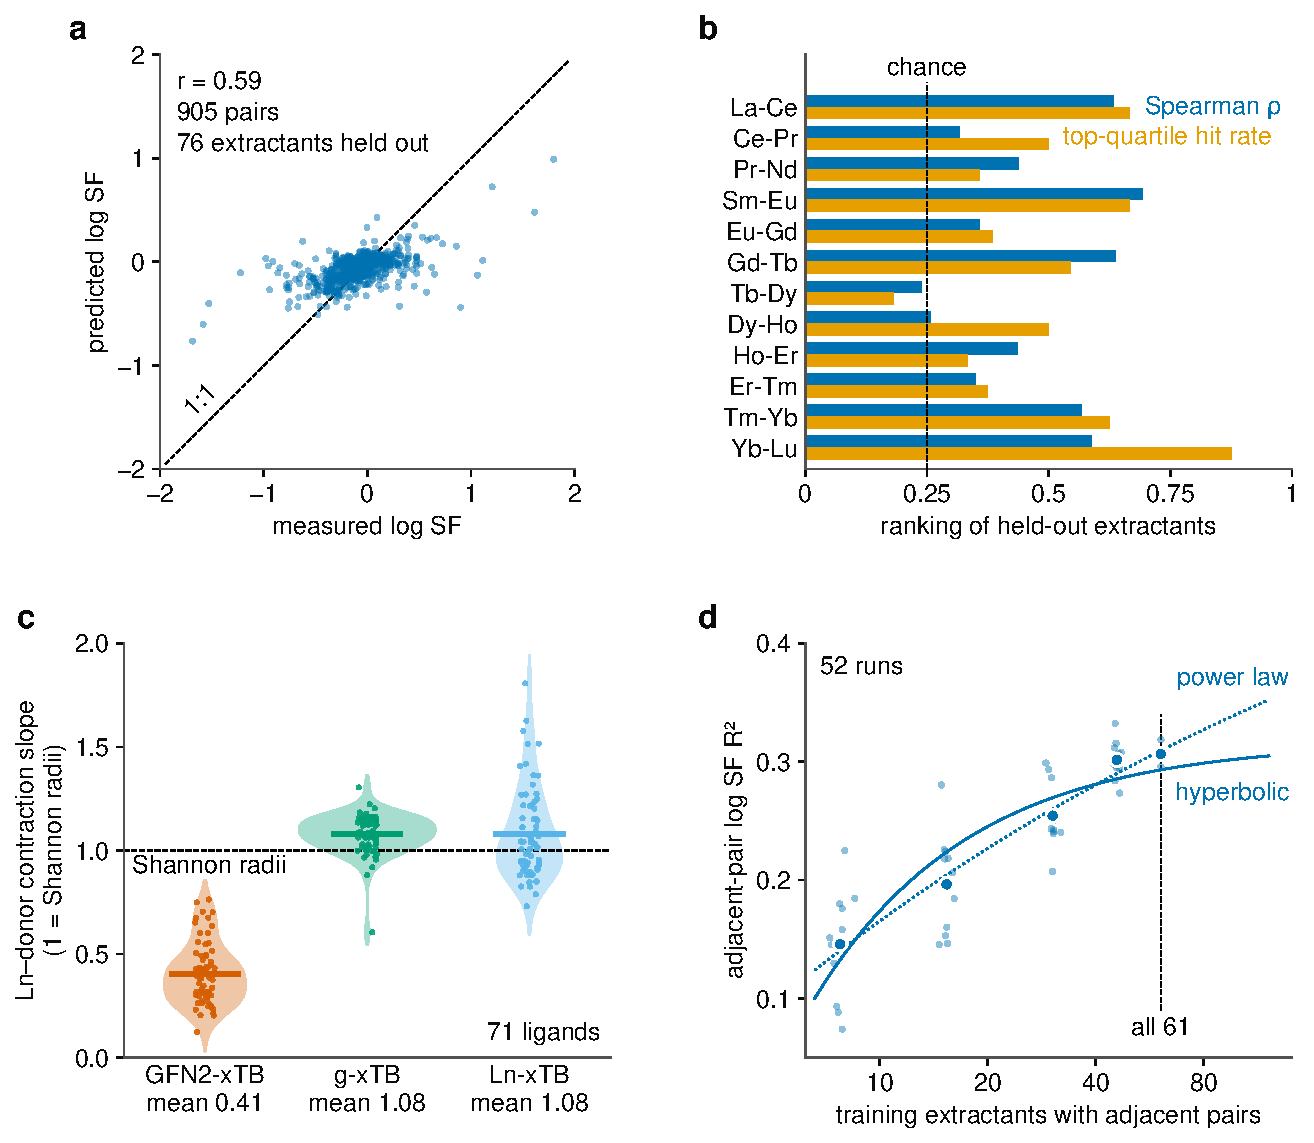
\includegraphics[width=\linewidth]{figure1}
  \caption{(a)~Predicted against measured adjacent-pair \logSF{} for the 905 pairs, extractants held out; the dashed line is the identity. (b)~Per adjacent pair: Spearman $\rho$ between predicted and measured extractant rankings, and the top-quartile hit rate against chance. (c)~Slope of the Ln--donor distance against the Shannon radius (the compliance \cL{}) for the 71 ligands under three Hamiltonians: points are ligands, shaded shapes their kernel density, bars the mean; 1 is exact agreement with the radii. (d)~Learning curve: small points are the 52 individual runs (four CV seeds, three nested draws) at their own training size, large markers the mean per fraction; solid and dotted lines the hyperbolic and power-law extrapolations; dashed line the full training set.}
  \label{fig:main}
\end{figure}

\begin{table}[t]
  \centering
  \caption{Adjacent-pair \logSF{} $R^2$ on the 905 pairs, extractants held out.}
  \label{tab:main}
  \begin{tabular}{lc}
    \toprule
    Model & $R^2$ \\
    \midrule
    CatBoost on \logD{} & $+0.268$ \\
    3D encoder, standalone & $+0.266$ \\
    Level + shape, Eq.~\eqref{eq:anchored} & $+0.318$ \\
    Level + shape + 3D shape, $w = 0.35$ & $\mathbf{+0.326}$ \\
    \bottomrule
  \end{tabular}
\end{table}

\paragraph{The correlation is robust and ligand-specific.}
On held-out extractants, predicted and measured separation factors correlate with $r = 0.59$ (Figure~\ref{fig:main}a). A cluster bootstrap over extractants gives an interval of $+0.21$ to $+0.38$ for $\adjR$. As a null test, the predictions were shuffled among extractants within each pair position. The shuffled predictions score $\adjR = -0.05$. Removing both the position means and the extractant means (10 and 13\,\% of the variance) leaves the ligand-by-position interaction, which is the selectivity itself. On this term the model still scores $+0.23$.

\paragraph{What the model is for.}
Ten percent of the pairs carry 71\,\% of the variance, so \adjR{} is mostly a statement about the large separations. Ranking the held-out extractants for each adjacent pair, the predicted top quartile contains a measured top-quartile ligand half of the time, against a quarter by chance, and the mean Spearman correlation with the measured ranking over the twelve positions is 0.46 (Figure~\ref{fig:main}b). As a detector of separations larger than a factor of two, which is one pair in five, the same predictions reach an AUC of 0.81. Split-conformal intervals \citep{vovk2005}, calibrated leave-one-extractant-out, cover 79\,\% and 90\,\% at nominal 80 and 90. The model is a triage tool: it says which ligand classes to consider for a pair and where their large separations lie; it does not rank ligands within one class, and that boundary is part of the claim.

\section{Three-dimensional structure: a small gain, and why it is small}
\label{sec:geom}
The optimised complexes enter the model through the shape channel only. When the encoder's block-centred prediction is blended with the tabular shape at $w = 0.35$, the score moves from $+0.318$ to $+0.326$ (eight CatBoost seeds, a 32-seed encoder ensemble). The difference is smaller than the seed-to-seed spread of a single encoder run (sd 0.0285), and it appears only when the network is restricted to the within-block differences: if the same geometry is reduced to 84 descriptor columns and given to a model that predicts \logD{} directly, the score falls from $+0.278$ to $-0.022$.

Why so little? Eight encoders were trained on these complexes with different architectures, neighbourhood cutoffs and losses, and they make essentially the same predictions: two disjoint eight-seed halves of one configuration agree at $r = 0.990$, ensembles of two different configurations at $0.986$, and the eight prediction vectors have an effective rank of 1.05. They all extract the same quantity: the ionic radius. GFN2-xTB fits parameters for cerium and lutetium and interpolates every lanthanide parameter linearly in $Z$ between them (largest residual $5.7 \times 10^{-7}$), so along the series an optimised metal--donor shell can respond to the metal only through a single scalar, which the tabular model already receives as a feature.

To measure how well that scalar is reproduced we substituted all fifteen lanthanides into one relaxed complex for each of 71 ligands, re-optimised under each Hamiltonian with the same binary and protocol, and regressed the mean metal--donor distance on the Shannon radius. The slope \cL{} is 1 when the complex contracts as the ionic radii do (Figure~\ref{fig:main}c). GFN2-xTB gives $\cL = 0.405 \pm 0.145$, that is, 40\,\% of the contraction. g-xTB \citep{gxtb}, which places the f electrons in the valence, gives $1.078 \pm 0.094$ and is closer to 1 for 70 of the 71 ligands. Ln-xTB \citep{lnxtb2026}, an element-by-element refit of the GFN2 lanthanide parameters, recovers the mean ($1.081 \pm 0.214$) but not a smooth series: a straight line explains 43\,\% of its metal dependence against 82\,\% for g-xTB, and it shows a 0.10~\AA{} dip at gadolinium in every ligand.

Correcting the contraction does not, however, give the model anything new. Replacing the GFN2-xTB geometries with g-xTB geometries changes the score by $+0.005$ ($p = 0.68$, eight paired seeds), and rebuilding the complexes in correspondence or relaxing them in solvent makes it worse (Appendix~\ref{app:controls}). Under all three Hamiltonians the ligand-specific part of the compliance is uncorrelated with the measured selectivity ($r = 0.11$, $-0.02$ and $0.17$ on 44 ligands); what changes from one Hamiltonian to the next is a profile shared by every ligand. The compliance test is cheap to run on any set of generated structures before an encoder is trained on them; if they respond to the metal through a single number, the encoder will learn nothing the radius does not already give.

\paragraph{How much data the problem needs.}
\label{sec:data-need}
Seventy-six extractants contribute scored pairs, yet the model is not starved. Trained on random fractions of the training extractants, the score rises from $+0.15$ with eight extractants to $+0.30$ with forty-six and then levels off at $+0.31$ with all sixty-one (Figure~\ref{fig:main}d). The last third of the data is worth $+0.005$, within seed noise, and the two fitted extrapolations put the gain from doubling the extractant count between $+0.01$ and $+0.04$. What the descriptors lack is whatever separates ligands inside one chemical class; adding americium data runs into the same limit (Appendix~\ref{app:am}).

\paragraph{Limitations and conclusion.}
No ceiling is identified: separations reproduce to about 0.16 log units on a spread of 0.22, but 70\,\% of the scored pairs have no replicate, and within one extractant the predicted shape of the series is weak. What the model does well is to say which ligands are selective and where their large separations lie, with calibrated uncertainty, for ligands it has never seen. The step that made this possible was asking for the shape of a series rather than its level.

\bibliographystyle{unsrtnat}
\bibliography{refs}

\appendix
\section{Protocol}
\label{app:protocol}
Code, out-of-fold predictions and every negative result: \url{https://github.com/mironovb/lanthanidestrain}.
\paragraph{Blocks.} The ten binned condition descriptors that define a block are acid class, acid strength, nitrate activity, pH, diluent family, modifier class, temperature, contact time, phase ratio and metal concentration. Pairs with a measured \logSF{} of exactly zero, which arise when both metals sit at a detection limit, are excluded. Promethium is absent, so Nd--Sm is not an adjacent pair.
\paragraph{Hyperparameters.} CatBoost: 1{,}500 iterations, learning rate 0.04, depth 9, $\ell_2$ regularisation 3, feature subsampling 0.3, quantile loss $\alpha = 0.6$, identical for the level and shape models. 3D encoder: width 96, three continuous-filter layers, 64 radial basis functions to 5~\AA{}, cutoff 4~\AA{}, heavy atoms only, dropout 0.15, head width 256, Adam at $2 \times 10^{-3}$ with weight decay $10^{-4}$, 60 epochs with early stopping on a validation fold, batches of 64 rows grouped by block so the contrast term always has pairs, pair-contrast weight 4 with adjacent pairs weighted $3\times$. Blend weight: nested selection over $\{0, 0.05, \dots, 1\}$ with equal weight per extractant.
\paragraph{Learning curve.} Fractions 0.125, 0.25, 0.5, 0.75 and 1 of each fold's training extractants, nested within a draw. The full-data run reproduces the stored champion exactly. Because the anchor is one number per extractant it cancels in every adjacent pair, so the level model does not affect the score and only the shape model's training set matters.

\section{Controls}
\label{app:controls}
Interventions under the same protocol on the 905 pairs; $\Delta R^2$ relative to the best comparable system.
\begin{center}
  \small
  \begin{tabular}{lc}
    \toprule
    Intervention & $\Delta R^2$ \\
    \midrule
    Simplicial encoder instead of the distance graph & 0.00 ($r = 0.96$, blend weight 0.01) \\
    Persistence descriptors as extra shape features & $-0.03$ to $-0.09$ \\
    Metal-feature weight $\times 2$ / $\times 5$ / $\times 10$ & $+0.00$ / $-0.05$ / $-0.08$ \\
    All-pairs difference model added to the blend & 0.00 \\
    Condition-transfer features & $+0.004$ \\
    g-xTB geometries instead of GFN2-xTB (802 complexes) & $+0.005$ ($p = 0.68$) \\
    Complexes rebuilt in correspondence & $-0.013$ \\
    Solvent-relaxed geometries, water / octanol & $-0.008$ / $-0.081$ \\
    GFN2 / g-xTB interaction-energy features & 0.00 \\
    \bottomrule
  \end{tabular}
\end{center}

\section{Ln-xTB parameters}
\label{app:lnxtb}
The Ln-xTB parameters are given in the supporting information of \citet{lnxtb2026} as PDF tables only. We parsed both copies (Tables S60--S61 and S62; no disagreement), replaced the $Z = 57$--$71$ blocks of the stock GFN2-xTB parameter file, and ran unmodified xtb 6.7.1. Single points on the 35 optimised structures shipped with the paper reproduce the published energies to better than $2 \times 10^{-8}$~$E_h$ once the paper's spin convention is used (the high-spin count of unpaired f electrons, reduced by one where its parity is inconsistent with the electron count). All 2{,}130 optimisations of the benchmark converged. A closed-shell control gives $\cL = 0.981 \pm 0.140$ with the same jagged series.

\section{Americium}
\label{app:am}
SAFE holds 1{,}794 Am(III) rows on 110 ligands, 95\,\% of them ligands with lanthanide data, giving 312 Am/Eu separation factors on 82 extractants under identical conditions. Zero-shot, with Am treated as a lanthanide at its radius, the Am/Eu separation is not predicted ($R^2 = -0.14$). Joint training with the Am rows reaches $+0.47$ on held-out extractants, but a control that assigns each held-out extractant the mean of the other extractants in its ligand family scores $+0.47$ as well, and within a family the model has no skill ($+0.02$); the lanthanide score is unchanged ($+0.002 \pm 0.020$ over paired seeds). The model learns which ligand classes discriminate Am from Eu, nothing finer.

\end{document}
